\documentclass{article}
\usepackage[utf8]{inputenc}
\usepackage{graphicx}
\usepackage{listings}
\usepackage[T1]{fontenc}
\begin{document}
\begin{titlepage}
\begin{center}
\line(1,0){350}\\
\huge{\bfseries Zaakpay SMS flow Document}
\line(1,0){250}\\
[1.5cm]
\textsc{\Large Version 1.0}
\end{center}


\end{titlepage}
\section{Login}

\begin{itemize}
\item To login, type your registered ID and password
\item Registered ID will have the format :

storeID@zaakpay.com
\item Default password is testing123
\end{itemize}
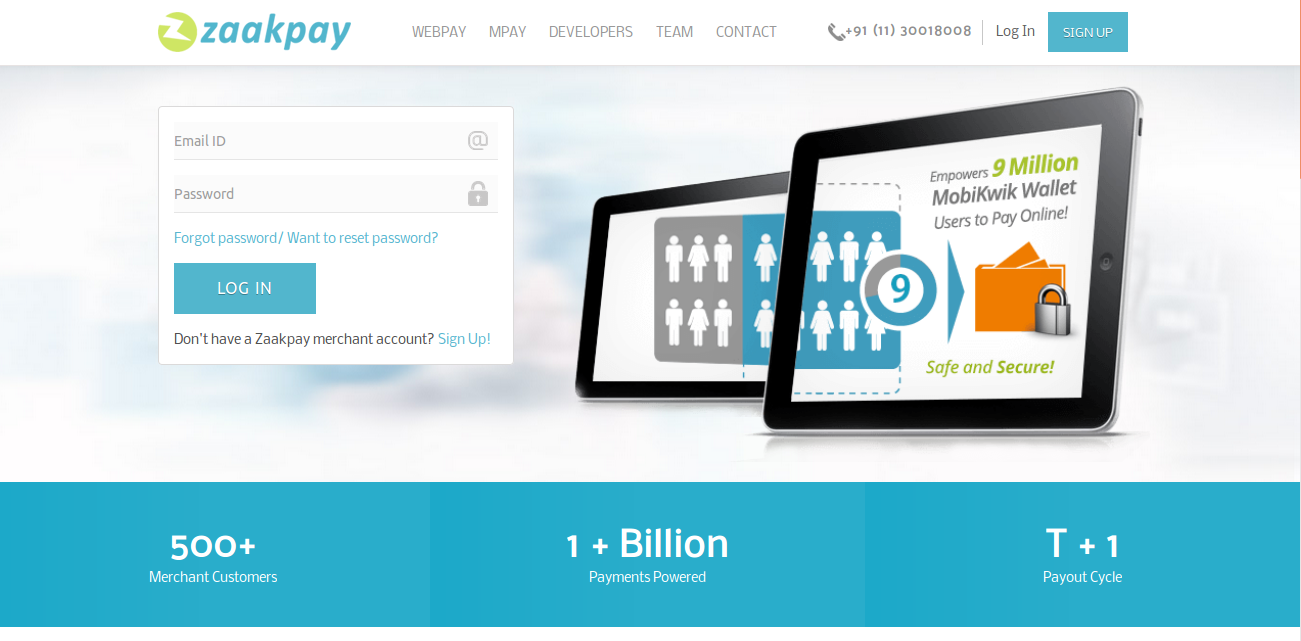
\includegraphics[width=6.5 in,height=4.4 in]{Login.png}
\newpage
\section{Change Credentials}
To change the password, do the below steps and refer the screenshots : 
\begin{itemize}
\item Click on settings tab
\end{itemize}
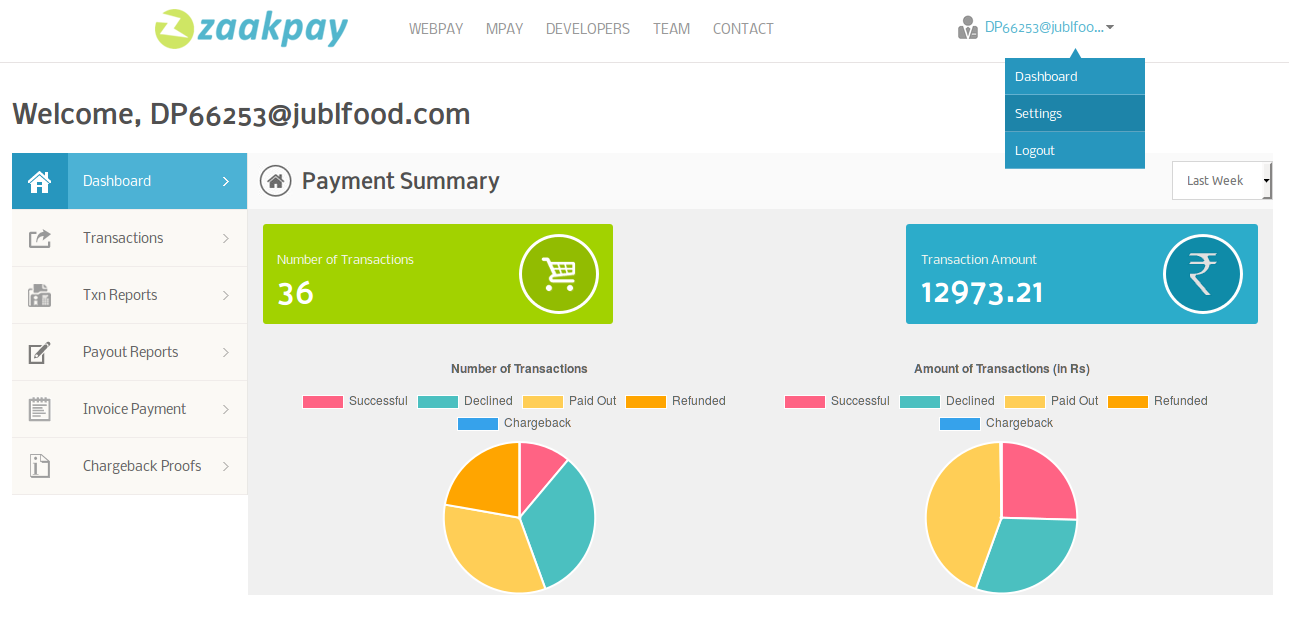
\includegraphics[width=6.5 in,height=3.4 in]{Settings.png}
\begin{itemize}
\item Click on "Change your password"
\end{itemize}
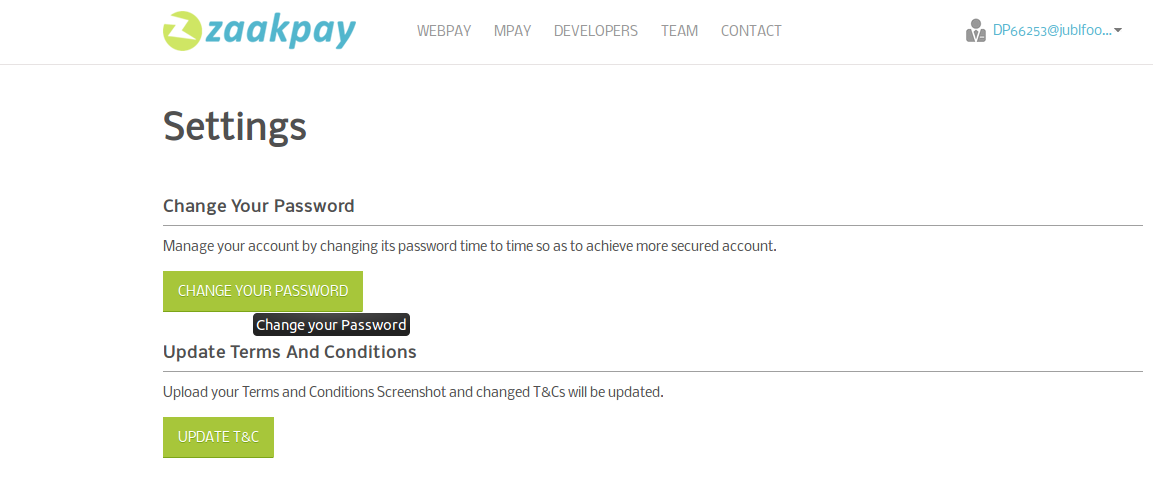
\includegraphics[width=6.5 in,height=2.4 in]{change_pass.png}
\newpage
\begin{itemize}
\item Enter the old password and new password
\end{itemize}
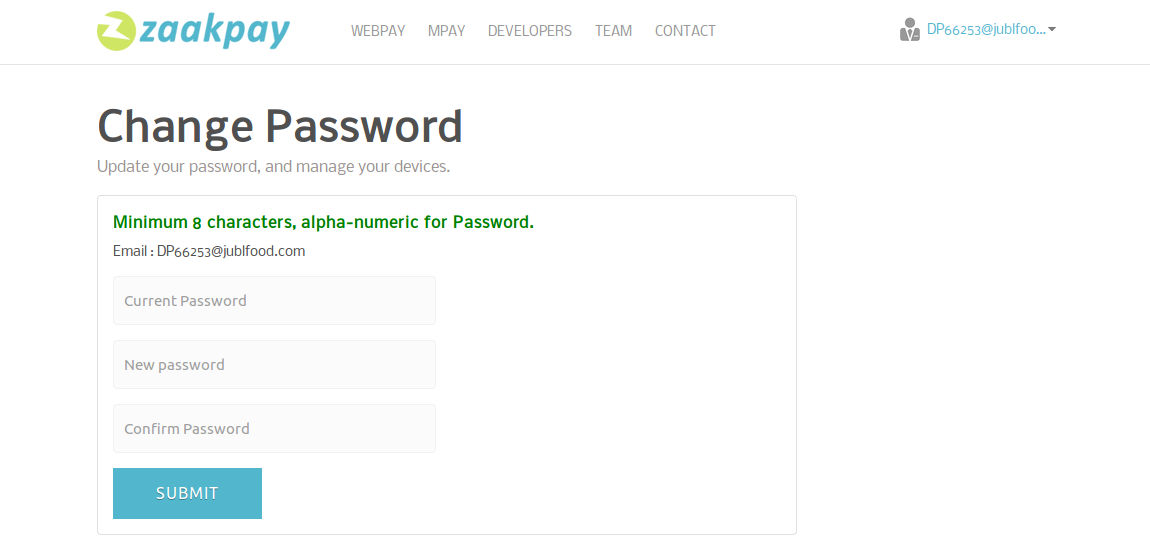
\includegraphics[width=6.5 in,height=3.4 in]{update_pass.png}
\newpage
\section{Dashboard}

After login, this is the view where the transactions can be viewed in a gist on the basis of :
\begin{itemize}
\item Number of transactions
\item Amount of transactions
\end{itemize}


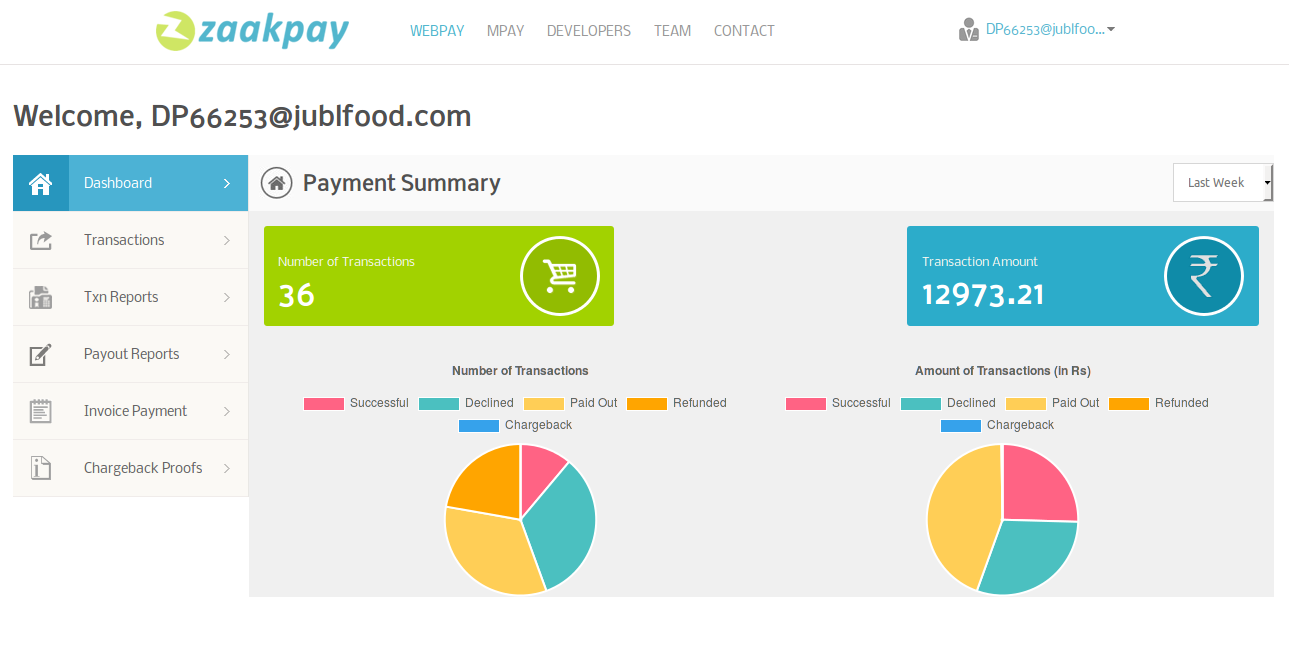
\includegraphics[width=6.5 in,height=3.4 in]{Dashboard_home.png}
\\
These features can be sorted for the current week, last week and last month.
\newpage
\section{Reports}

\subsection{Transaction Reports}
 In the transaction section, you can search the transactions on the basis of
\begin{itemize}
\item Date
\item Email ID
\item Order ID
\item Status
\end{itemize}
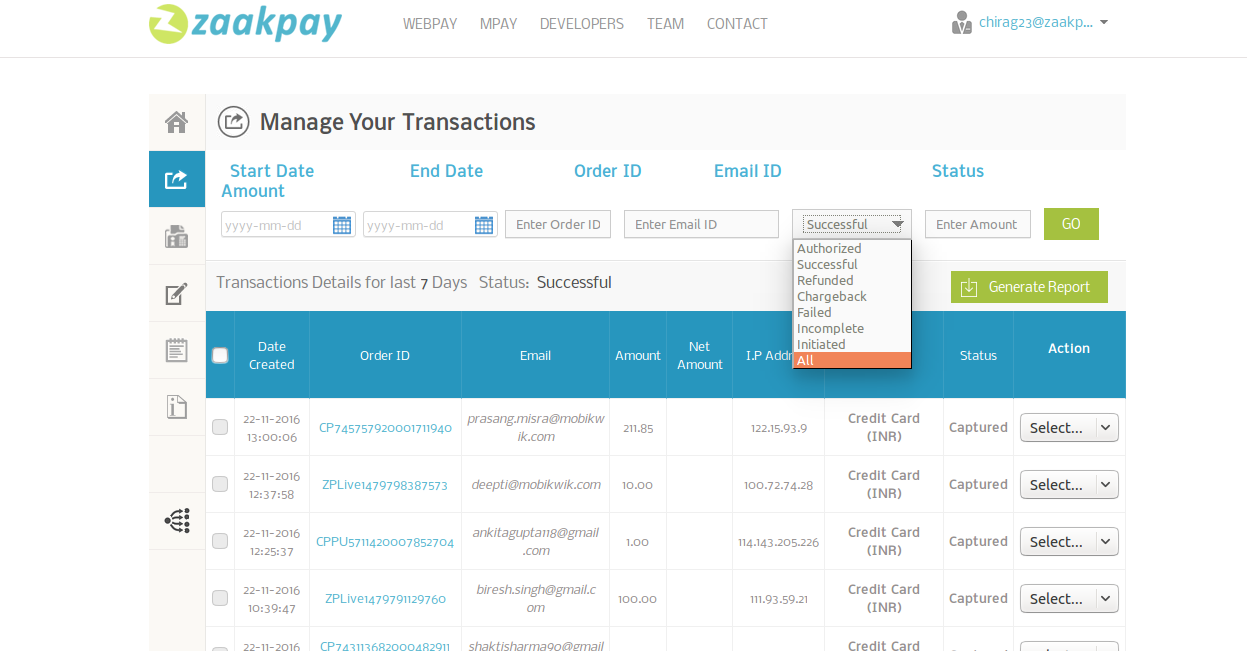
\includegraphics[width=6.5 in,height=3.4 in]{transactions.png}
\newpage
Any transaction can be in the following states :
\begin{itemize}

\item SMS Status

This state is when the payment link is pushed to the customer. This has a time to live for 15 minutes after which the link would expire \\
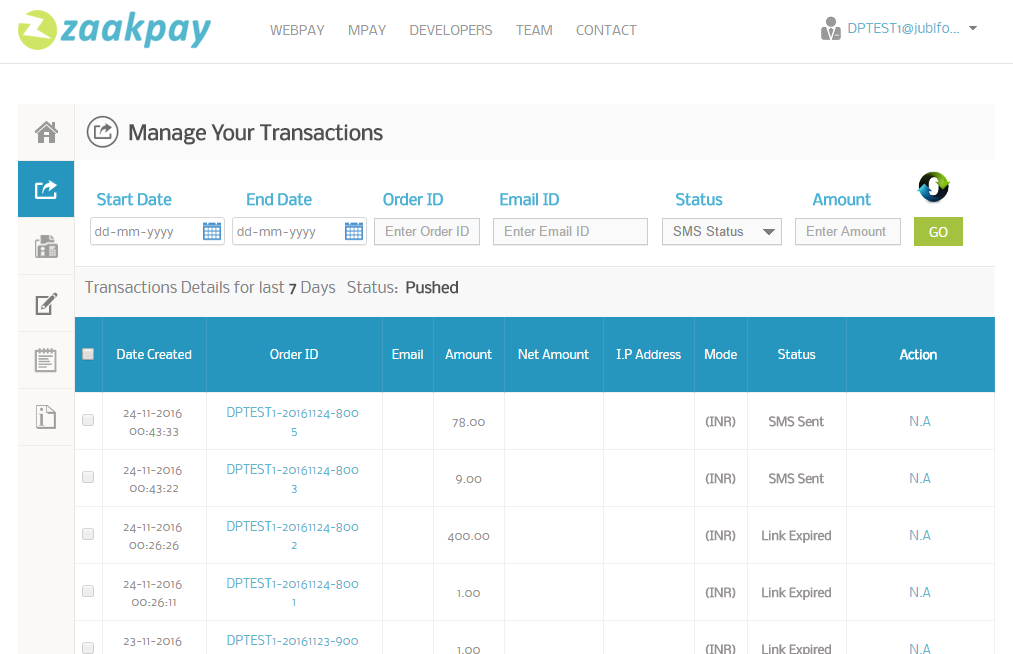
\includegraphics[width=6.5 in,height=3.4 in]{sms_sent.png} \\
This state has the following sub-states:
\begin{itemize}
\item SMS Sent

When a merchant sends a request to a customer, the order ID can be seen in this state. This state will be valid for 15 minutes. Post that the order ID can be shifted to "Link Expired" or "Initiated"
\item Link Expired

After 15 minutes of inactivity by the customer, this will be the status of the order ID 



\end{itemize}
\newpage
\item Initiated

If customer clicks on the link and reaches the payment gateway page, the status becomes initiated. If customer is inactive till 15 minutes, the status will change to "Declined", else, it will be processed further
\item Successful

The transaction is complete and successful
Under this category, the sub categories are :
\begin{itemize}

\item Captured

The transaction amount is captured and will be paid to the merchant

\item Payout Initiated

The transaction amount is ready for transfer to the merchant's bank account
\item Payout Completed

The transaction amount is transferred to the merchant's bank account


\item Settled 

The bank has confirmed that the valid transactions have been credited 
\end{itemize}
\item Failed

This means that due to some reasons the payment was not successful or the customer could not complete the payment within 15 minutes of the bill pushed


\item Refunded

The transaction is successfully refunded

\newpage

\end{itemize}
\newpage
\subsection{Payout Reports}

Whenever the payout is generated, the reports can be downloaded from this section

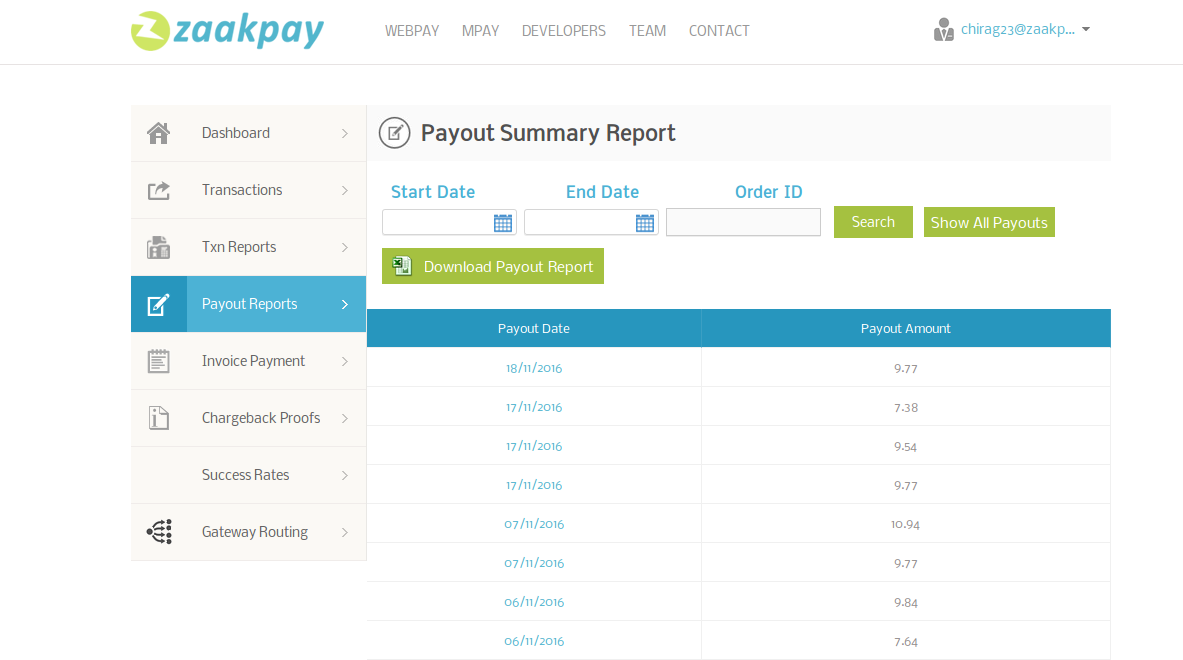
\includegraphics[width=6.5 in,height=3.4 in]{payout_report.png}
\end{document}
